\documentclass[]{article}
\usepackage{graphicx}
\graphicspath{ {./images/} }
\usepackage{caption}
\usepackage{subcaption}
\usepackage{amsthm}
\usepackage{amsfonts}
\usepackage{amsmath}
\usepackage{amssymb}
\usepackage{mathrsfs }
\usepackage[ruled,linesnumbered]{algorithm2e}
\newtheorem{mydef}{Definition}[section]
\newtheorem{mytheorem}{Theorem}[section]

%opening
\title{Master Thesis --  Math Formalization}
\author{Kefang Ding} 
\date{\today}

\begin{document}

\maketitle

\hrulefill
\hrulefill 

\begin{abstract}
This article describes the work we have done so far. The following sections are organized in this way. Section 1 describes the problems to solve. Section 2 introduces formal definitions for dfg-method and adding long-term dependency. Section 3 gives details of the algorithm steps. 
\end{abstract}

\section{Introduction}
The inputs for process model repair include one existing process model, a corresponding event log and a set of KPIs for the data evaluation in event log. After evaluating event log by KPIs, positive and negative labels are assigned on each trace in event log file. 

In state-of-the-art technologies in process mining, only positive traces are used to repair model, while negative information is omitted. In this way, the generated models tend to have low precision. In order to increase the precision, we adapt Inductive Miner algorithm on the base of directly-follows relation of activities. This algorithm, called dfg-algorithm, uses both positive and negative information from event log and generates a model with high fitness. Yet after application, dfg-algorithm cannot discover, change the long-term dependency in the model, so that the model still has less precision. With concept long-term dependency, it describes the dependency between activities, where the execution of one activity affects the execution of another activities later. Later, we investigate problem and propose one algorithm to add long-term dependency constraints in model. 
%% we have the model of Petri net from 

In this article, we propose one algorithm which combines dfg-method and adding long-term dependency programs, to incorporate negative information. The architecture of this model repair algorithm is as shown in Figure \ref{fig:architecture_blackbox}.
\begin{figure}[!h]
	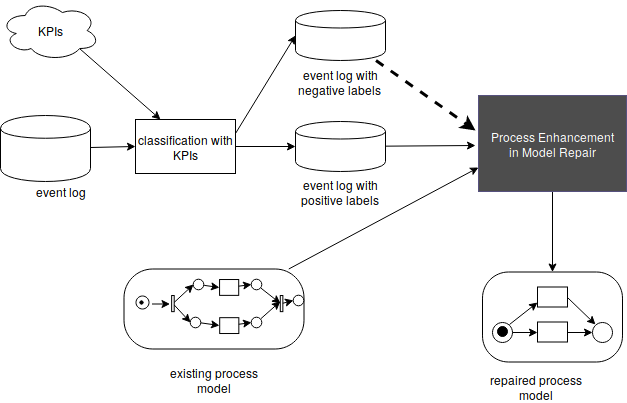
\includegraphics[width=\textwidth]{FD00_approach_blackbox.png} 
	\caption[Model Repair Architecture]{Model Repair Architecture -- \small firstly, event log is divided into positive and negative logs according to KPIs. Later, they are passed as inputs into repair process with existing process model. The output of this process is repaired model.}
	\label{fig:architecture_blackbox}
\end{figure}
%% some explanation about this architecture.

\section{Definitions}
\subsection{Definitions Related To Dfg-Method}
In this part, we provides concepts related to the dfg-method which is based on directly-follows graph. A directly-follows graph as used in \cite{leemans2013discovering}, represents the directly-follows relation of activities in event log. For instance, if there are traces of $\langle ...,A,B,... \rangle$ in event log, one edge (A,B) is added into directly-follows graph. By cutting directly-follows graph under different conditions, Inductive Miner\cite{leemans2013discovering,leemans2014discovering} discovers a process model. Unlike this process, we adapt Inductive Miner to repair model by using existing model, and event log with labels.
 
\begin{mydef}[Cardinality in directly-follows graph]
	Given a directly-follows graph G(L) derived from an event log L, the cardinality of each directly-follows relation in G(L) is defined as:  
	\begin{itemize}
		\item $Cardinality(E(A,B))$ is the frequency of traces with $\langle ...,A,B,... \rangle$. 
		\item Start node A cardinality $Cardinality(Start(A))$ is the frequency of traces with begin node A.
		\item End node B cardinality $Cardinality(End(A))$ is the frequency of traces with end node B.
	\end{itemize}	
\end{mydef}
From the positive and negative event log, we can get directly-follows graphs, respectively $G(L_{pos})$ and $G(L_{neg})$. Each edge of  $G(L_{pos})$ and $G(L_{neg})$ has a cardinality to represent the strength of this directly-follows relation. 
However, when the existing model is transformed into  directly-follows graph $G(L_{ext})$, there is no point to assign cardinality on each edge. So we just set 1 to cardinality of each edge. 

%To incorporate all information from  $G(L_pos)$, $G(L_neg)$ and $G(L_ext)$, a data structure is defined directly-follows matrix. 
To incorporate all information from  $G(L_{pos})$, $G(L_{neg})$ and $G(L_{ext})$, we define  weight for each directly-follows relation in graph. 
\begin{mydef}[Weight of directly-follows relation]
	Given a directly-follows graph G(L), the weight of each directly-follows relation is defined as \[ Weight(E(A,B)) = \frac{Cardinality(E(A,B))}{Cardinality(E(A,*))}  \] 
	for start activities A, we have 
	\[ Weight(Start(A)) = \frac{Cardinality(Start(A))}{Cardinality(Start(*))} \]
	Similarly for end activities B, we have
	\[ Weight(End(B)) = \frac{Cardinality(End(B))}{Cardinality(End(*))} \]
	E(A,*) means all edges with source A, E(*,B) means all edges with target B, Start(*) represents all start nodes, and End(*) represents all end nodes.
\end{mydef}
After defining the weights of each directly-follows relation, for each directly-follows relation, there are three weights from $G_{pos}$, $G_{neg}$ and $G_{ext}$. The following strategy assigns new weight to directly-follows relation to new generated directly-follows graph $G_{new}$.
\begin{mydef}[Assign new weights to graph $G_{new}$]
	there are three weights from $G_{pos}$, $G_{neg}$ and $G_{ext}$, the new weight is 
	\begin{itemize}
		\item For one directly-follows relation, \[ Weight(E_{G_{new}}(A,B)) = Weight(E_{G_{pos}}(A,B)) + Weight(E_{G_{ext}}(A,B)) - Weight(E_{G_{neg}}(A,B))\]
		\item For start activities A, we have 
		\[ Weight(Start_{G_{new}}(A)) = Weight(Start_{G_{pos}}(A)) + Weight(Start_{G_{ext}}(A)) - Weight(Start_{G_{neg}}(A)) \]
		\item For end activities B, we have
		\[ Weight(End_{G_{new}}(A)) = Weight(End_{G_{pos}}(A)) + Weight(End_{G_{ext}}(A)) - Weight(End_{G_{neg}}(A)) \]
	\end{itemize}
\end{mydef}
After assigning all the weight to directly-follows relation in $G_{new}$, we filter out all directly-follows relation in $G_{new}$ with weight less than 0. 
Then, we transform the $G_{new}$ into process tree bu using Inductive Miner for the next stage.

\subsection{Definitions Related To Add Long-term Dependency}
\textit{Example 1} Consider event log L with labels \[L =[\langle A,C,E \rangle^{50,pos}, \langle B,C,D \rangle^{50,pos}, \langle A,C,D \rangle^{50,neg}]. \] $\langle A,C,E \rangle^{50,pos}$ means there are 10 traces $\langle A,C,E \rangle$ labeled as positive in event log. Similarly, $\langle A,C,D \rangle^{50,neg}$ represents there are $\langle A,C,D \rangle$ traces at number 50 in event log which have negative labels. 

After applying the dfg-algorithm, a model as shown in Figure \ref{fig:pn_without_lt_exm01} is discovered. In event log L, B and D has long-term dependency, and A is expected to support only the execution of E, since $<A,C,D>$ is negative and $<A,C,E>$ is positive. However, the model doesn't express those constraints.
\begin{figure}[h!]
	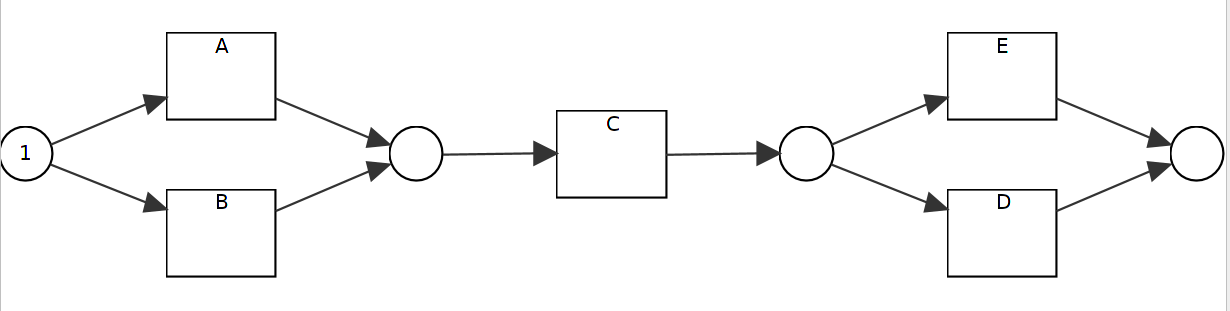
\includegraphics[width=\textwidth]{PN06_Seq_2_xor_notnested.png}
	\caption{Process model generated from dfg-algorithm}
	\label{fig:pn_without_lt_exm01}
\end{figure}
Obviously, long-term dependency relates the choices structure in process model, such as exclusive choice, loop and or structure. Due to the complexity of or and loop structure, only the long-term dependency in exclusive choice is considered. 

The inputs for this algorithm are,
\begin{itemize}
	\item Repaired model in process tree
	\item Event log with positive and negative labels
\end{itemize}
The output of this algorithm is: 
\begin{itemize}
	\item Repaired model in petri net with long-term dependency
\end{itemize}
%%if now, we only consider the repaired process tree model, then we don't have problems to make the weights of dfg and long-term dependency unified. But we have it from the existing model, because of existing factor. 
%% Now we have the firstly-repaired model, if we want to create long-term dependency, we also have the 3 weights:: 
%% Ext_Wlt(Si, Tj), but when our negative factor affects, we need to unify them!!To prove it!!! 

Process tree, as one input for the algorithm, is one common model to interpret business process in process mining. It's a block-structured tree. To specify the process tree with respect to long-term dependency, the following definitions are in need. Firstly, the definitions related to tree are reviewed.
\begin{mydef}[Tree]
	Let $ \mathscr{E} $ be a finite set of entities, a tree is a collection of entities called nodes, which are connected by edges. A tree T is,
	
\begin{itemize}
	\item t, with  $t\in \mathscr{E}$, t has no outgoing edges
	\item $t(T_1,T_2,...,T_n)$, with $t\in \mathscr{E}, i,n\in \mathbb{N}, i \leq n ,T_i$ is a tree.
\end{itemize}
\end{mydef}
$T_i$ is a child or subtree of $t(T_1,T_2,...,T_n)$, $t(T_1,T_2,...,T_n)$ is one parent of $T_i$, which can be expressed in $P(t(T_1,T_2,...,T_n),T_i)$. The root of tree is the node without any parent; A tree has only one root. A leaf node is the node which has no children nodes.\\
For a node in a tree, its ancestor and descendant are defined as:
\begin{mydef}[Ancestor Relation Anc(A,t)]
	An ancestor of a node t in a tree is a node A, written as $ Anc(A,t) \Rightarrow True$, if those conditions hold,  
	\begin{itemize}
	\item A is a parent of t, written as $ P(A,t) \Rightarrow True$, or
	\item $\exists t_1,t_2..t_n,n\in \mathscr{E}, i < n, P(A,t_1)\land P(t_i,t_{i+1}) \land P(t_n,t) \Rightarrow True $
   \end{itemize}
\end{mydef}
The ancestor of root is empty, while leaf nodes has no descendants. Based on this, we define the ancestors set of a node s. 
\begin{mydef}[Ancestors of a node a]
	The ancestors set of a node s, Ancestors(s), is defined as: \[ Ancestors(A)=\{t|Anc(t,s) \Rightarrow True \} \]
\end{mydef}
Accordingly, descendant relation is given for node t and node s, Des(s,t). If node s is the ancestor of t, then t is a descent of s. $Anc(s,t) \Rightarrow Dec(t,s)$; The set of descendants of node t is Descendants(t).
\begin{mydef}[Least Common Ancestor]
	A least common ancestor for node $s$ and node $t$ in a tree is a node n, where 
	\[Anc(n,s) \land Anc(n,t) \land \exists! m Anc(n,m) \land Anc(m,s) \land Anc(m,t) \]
\end{mydef}

In process tree, all the leaves are activities in business process, and the middle nodes are operators which represents the relations of all its children nodes\cite{vanderAalst:2016:PMD:2948762,leemans2013discovering}. This paper uses four operators in context of long-term dependency. The four relations.  $\{\rightarrow, \times, \land, \circlearrowright\}$ are considered. 

Next, we only focus on exclusive xor structure on long-term dependency. As known, long-term dependency is associated with choices. In xor block, it means the choices of each xor branch in xor block. For sake of convenience, we define the xor branch.

$Q= \times(Q_1 , Q_2 ,.. Q_n)$, $Q_i$ is one xor branch with respect to Q, rewritten as $XORB_{Q_i}$ to represent one xor branch $Q_i$ in xor block, and record it $XORB_{Q_i} \in XOR_{Q}$. For each branch, there exists the begin and end nodes to represent the beginning and end execution of this branch, which is written respectively as Begin($XORB_{Q_i}$) and End($XORB_{Q_i}$).

%% but the structure of xor branch, do we need to think of right now?? we need to think of it 
For convenience of analysis, two properties of xor block, purity and nestedness are demonstrated to express the different structures of xor block according to its branches.
\begin{mydef}[XOR Purity and XOR Nestedness] The xor block purity and nestedness are defined as following: \\
	\begin{itemize}
		\item A xor block $XOR_Q$ is pure if and only $\forall XORB_X \in XOR_Q, XORB_X $ has no xor block descent, which is named as pure xor branch. Else,
		\item A xor block $XOR_Q$ is nested if $ \exists XOR_X, Anc(XOR_Q, XOR_X) \rightarrow True  $. Similarly, this xor branch with xor block is nested.
	\end{itemize}
\end{mydef}
%% change the graph for whole explaination!!
In the Figure\ref {fig:xor_nested_branch_variants}, xor block Xor(c1,c2) are pure and not nested, since all the xor branches are leaf node, but xor block Xor(a,Seq(b,Xor(c1,c2))) is impure and nested with Xor(c1,c2). 
\begin{figure}[h!]
	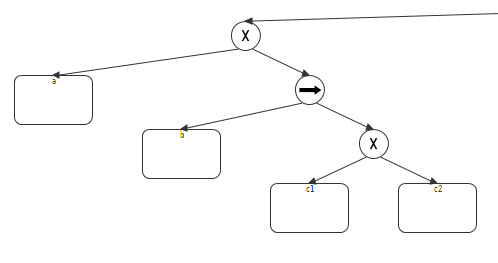
\includegraphics[width=\textwidth]{PT02_xor_nested_and_pure.png}
	\caption{XOR branch variants}
	\label{fig:xor_nested_branch_variants}
\end{figure}

%% xor branch, the dependency between them, then how about the dependency on that part, does it exist in the xor block, so we can define it ??
%% the full completeness is also dependency, but sth different, 
%% for arbitrary two xor branches, if they are long-term dependency?? Can I decide, or not ?? I can decide it!! But in the specific way, if they are in a pair, they are ok, else, not !!! 
%% but it goes far, so only write down what I have achieved, but in their thinking way, why in my way?? 
%% given two branch, and they have order, just complexity of implementation, then we only consider the directly ones!!  

Long-term dependency researches on the dependency of choices in xor block, with observation, actually on the pure xor branch, because nested xor branch has multiple choices, which affect the execution of later process. For two arbitrary pure xor branches, to have long-term dependency, they firstly need to satisfy the conditions: (1) they have an order;(2) they have significant correlation.
The order of xor branch follows the same rule of node in process tree which is explained in the following.
\begin{mydef}[Order of nodes in process tree]
	Node $X$ is before node $Y$, written in $X \prec Y$, if $X$ is always executed before $Y$.  In the aspect of process tree structure, $X \prec Y$, if the least common ancestor of $X$ and $Y$ is a sequential node, and $X$ positions before $Y$.
\end{mydef} 
%% how to define the correlation fo xor branches, if they always happen together
The correlation of xor branches is significant if they always happen together. To define it, several concepts are listed at first. 
\begin{mydef}[Xor branch frequency]
	Xor branch $XORB_X$ frequency in event log l is $F_{l}(XORB_X)$, the count of traces with the execution of $XORB_X$. \\
	For multiple xor branches, the frequency in event log l is defined as the count of traces with all the execution of xor branches $XORB_(Xi)$ , written as \[F_{l}(XORB_(X1), XORB_(X2),...,XORB_(Xn))\].
\end{mydef}
%% correlation means the two always happen together, if one not shown, the other also not?? So the connection support.. how to define them?? 
%% connection support, we can say only on number, when it is over one value, 
After calculation of the frequency of the coexistence of multiple xor branches in positive and negative event log, we get the supported connection of those xor branches, and define the correlation. 
\begin{mydef}[Correlation of xor branches]
For two pure xor branches, $XORB_X \prec XORB_Y$, the supported connection is given as \[SC(XORB_X,XORB_Y)= F_{pos}(XORB_X, XORB_Y) -F_{neg}(XORB_X, XORB_Y)\]. If $SC(XORB_X,XORB_Y) > lt-threshold$, then we say $XORB_X$ and $XORB_Y$ have significant correlation.
\end{mydef}
% here we argue why they must be directly-follows relation
Under above concepts, if $XORB_X \prec XORB_Y$ and they have significant correlation,  $XORB_Y$ is potentially dependent on  $XORB_X$. In general cases, between $XORB_X$ and $XORB_Y$ there exists one $XORB_Z$, which potentially depends on $XORB_X$; At the same time, $XORB_Y$ is also dependent on $XORB_Z$ with certain potent. In our work, the crossed dependency of $XORB_X$ and $XORB_Y$ is ignored, we only consider the directly potential dependency, which requires $XORB_X$ is directly-followed by $XORB_Y$. 
\begin{mydef}[Directly-followed relation of xor branch]
	$XORB_X$ is directly-followed by $XORB_Y$, $XORB_X \leq XORB_Y$ if 
	\[ \exists ! XORB_Z, \: XORB_X \prec XORB_Y \land XORB_X \prec XORB_Z \land XORB_Z \prec XORB_Y \]
\end{mydef}
% Also, the amount of loan also decides the check later. If it is small, the report to manager and the check of finance is not necessary.

% here we argue why they are multiple relation;;
During the execution of a process model in reality, several choices decide one choice later, and one choice decides many choices later. For example, to apply the loan, only if the credit is fine, and the amount of loan is affordable, the loan is possible to give; else it is declined. Therefore, it is not meaningful to only consider the binary long-term dependency of xor branches. We expand the binary long-term dependency into multiple relation. 
\begin{mydef}[long-term dependency on set of xor branches]
	\label{def: branches-final-lt}
	Two set of xor branches ${XORB_{X1}, XORB_{X2}..., XORB_{Xm}}$, ${XORB_{Y1}, XORB_{Y2}..., XORB_{Yn}}$ have long-term dependency, if 
	\[\forall XORB_{Xi},XORB_{Yj}, XORB_{Xi} \leq XORB_{Yj} \] and
	\[SC({XORB_{X1}, XORB_{X2}..., XORB_{Xm}}, {XORB_{Y1}, XORB_{Y2}..., XORB_{Yn}}) > threshold  \]
\end{mydef}
${XORB_{X1}, XORB_{X2}..., XORB_{Xm}}$ depend the execution of ${XORB_{Y1}, XORB_{Y2}..., XORB_{Yn}}$. 


\section{Algorithm Implementation}
After combining this algorithm, the algorithm is completed to incorporate negative information to repair model as shown in Figure \ref{fig:architecture}.
\begin{figure}
	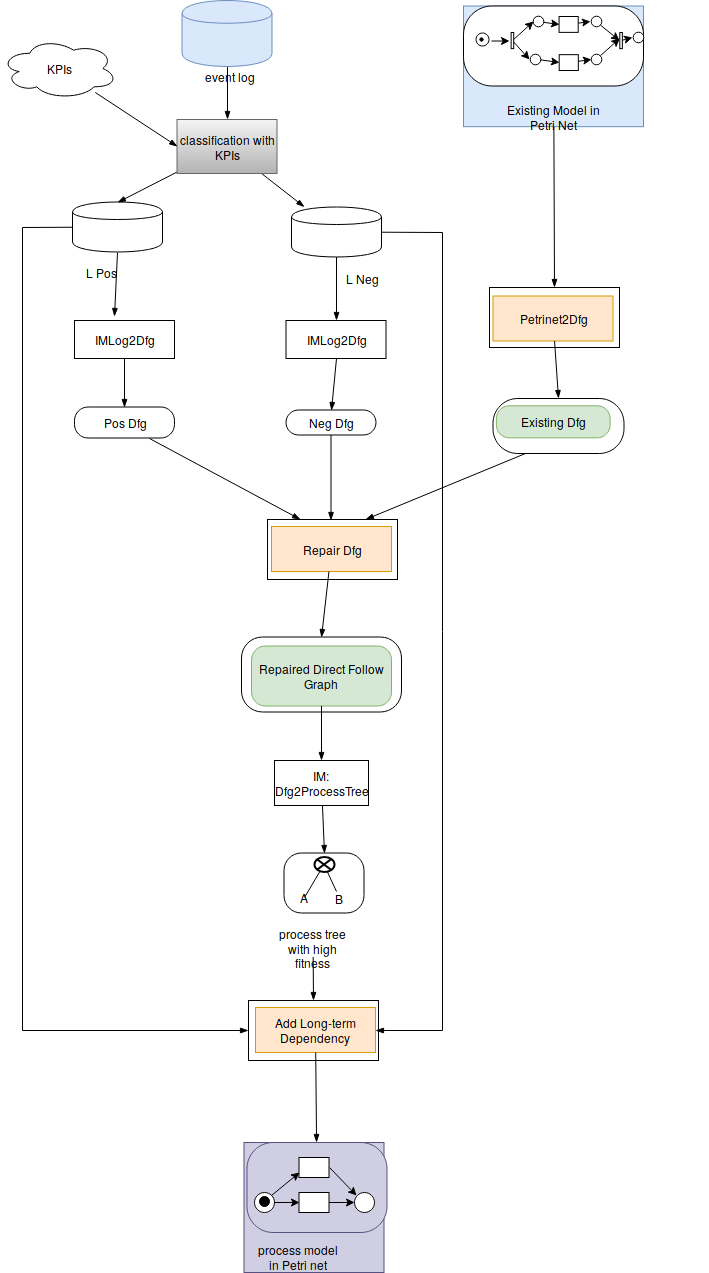
\includegraphics[width=\textwidth, height=\textheight]{FD_architecture_detail_02.png}
	\caption[Model Repair Architecture]{Model Repair Architecture -- \small Rectangles represents processes and output data in eclipse shape, especially customized processes and data are in doubled lattice shape. Input event log and existing model are in blue, KPIs are in cloud. The output is a petri net in purple. }
	\label{fig:architecture}
\end{figure} 
\subsection{Detect the long-term dependency of xor branches}
According to Definition \ref{def: branches-final-lt}, it gives constrains on xor branches. In term of process tree structure, constrains are:
\begin{itemize}
	\item xor blocks where the xor branches belong to are also directly-followed; Only they are able to create xor block pair. 
	\item the combination of potentially long-term dependency in xor blocks is not complete. If complete, any xor branch can go to next branches, the structure keep the same; So no necessary is required to add places and transitions to connect the xor branches. 
\end{itemize}
With this knowledge, we develop Algorithm \ref{alg: detect-lt} to detect the long-term dependency. 
\begin{algorithm}
	\SetAlgoLined
	\label{alg: detect-lt}
	\KwResult{Discover Long-term Dependency In Model}
	create a list including all xor pairs in process tree\;
	\While{pair in xor pair list}{
		generate all the combination of xor branches set \;
		check the all set if they have potential long-term dependency
		\If{this pair has complete long-term dependency combination}{
			remove this pair from xor pair list\;
		}{
			keep the pair in list
		}
	}
	transfer process tree into Petri net\;
	add long-term dependency in petri net\;
	\caption{General steps to add long-term dependency}
\end{algorithm}
The subprogram to generate the set of xor branches is in a brutal way.
\begin{algorithm}
	\SetAlgoLined
	\label{alg: generate-lt-combination}
	Given two set of xor block $A={XOR_{A1} ,XOR_{A2}, ...XOR_{Am}}$ and $B={XOR_{B1} ,XOR_{Bn}, ...XOR_{Bn}}$ with $A$ is directly-followed by $B$.
	create a list to store the xor branches
	
	\caption{Generate combination of xor branches}
\end{algorithm}
% after this, we need to ?? 

\subsection{Add long-term dependency on Petri net}
After detecting long-term dependency on xor branches from process tree, silent transitions and extra places are added to express those dependency on Petri net. Given, the basic idea is to add places after $XORB_X$ and places before $XORB_Y$, then connect the places by silent transition. Due to the structure of xor branches, situations differ, as listed in the Algorithm \ref{alg: Adding method}.  %% some simple examples are given to address those problem
\begin{algorithm}
	\SetAlgoLined
	$XORB_Y$ is dependent on $XORB_X$\;
	\If{$XORB_X$ is leaf node}{
		One place is added after this leaf node. \;
	}
	\If{$XORB_X$ is Seq}{
		Add a place after  the end node of this branch;\;
		The node points to the new place;\;
	}
	\If{$XORB_X$ is And}{
		Create a place after the end node of every children branch in this And xor branch; \; 
		Combine all the places by a silent transition after those places; \;
		Create a new place directly after silent transition to represent the And xor branch; \;
	}

	\If{$XORB_Y$ is leaf node}{
		One place is added before this leaf node. \;
	}\If{$XORB_Y$ is Seq}{
		Add a place before  the end node of this branch;\;
		The new place points to this end node;\;
	}\If{$XORB_Y$ is And}{
		Create a place before the end node of every children branch in this And xor branch; \; 
		Combine all the places by a silent transition before those places; \;
		Create a new place directly before silent transition to represent the And xor branch; \;
	}
    Connect the places which represent the $XORB_X$ and $XORB_Y$ by creating a silent transition.
	\caption{Add long-term dependency between pure xor branch}
	\label{alg: Adding method}
\end{algorithm}

\pagebreak
\bibliography{bibtex2ref.bib}
\bibliographystyle{ieeetr}
\end{document}
